% Just ignore everything between this and the next commented line!

\documentclass[12pt]{article}
 \usepackage[margin=1in]{geometry} 
 \usepackage[usenames,dvipsnames]{xcolor}
\usepackage{amsmath,amsthm,amssymb,amsfonts, 
hyperref, color, graphicx,ulem}
\usepackage{datetime}
\usepackage{subcaption}
\newcommand{\N}{\mathbb{N}}
\newcommand{\Z}{\mathbb{Z}}
\newcommand{\Q}{\mathbb{Q}}
\newcommand{\mm}{\textcolor{blue}{You need to use math mode whenever you are writing logic symbols, variables, sets etc. and you need to use text whenever you are writing words. If you are not sure what this means, please speak to me.}}
\newcommand{\al}{\textcolor{blue}{You might try the align environment as shown below: 
\begin{align*}
y=&a+b+a\\
=&2a+b
\end{align*}
The \& symbol allows you to line up the ='s or anything else you want to line up! It also saves you the space between lines of display style equation!}}
\newcommand{\steps}{\textcolor{blue}{You need to use the claim environment to give a claim, then close that and use the proof environment to give your proof.}}
\newcommand{\nproof}{\textcolor{blue}{I see what you are trying to say, but this is not a proof. Please see me if you do not understand what I mean by this.}}
\newcommand{\equal}{\textcolor{blue}{You can only use ``='' between two things which are actually equal. This is not just a way of stringing things together!}}
\newcommand{\mul}{\textcolor{blue}{This is not a valid way of denoting multiplication. You can use $\times$ or $\cdot$, or often the implied multiplication of adjacent variables.}}
\newcommand{\ex}{\textcolor{blue}{You cannot just give one example. You are tasked with showing that this claim holds for all possible values.}}
\newcommand{\thus}{\textcolor{blue}{``therefore'', ``thus", and other words of this flavor should be used only when the preceding sentence leads us to the following sentence. It is not just a way to string things together!}}
\newcommand{\words}{\textcolor{blue}{You need punctuation and words. Remember a proof is supposed to walk the reader through your thought process.}}
\newcommand{\order}{\textcolor{blue}{As a general rule, if the sentences can be reorganized and the proof doesn't make significantly less sense, then it is probably not very well structured! The arguments should flow into each other. Generally sentences should justify each other and you should feel like you are building one thought on top of another.}}
\newcommand{\pr}{\textcolor{blue}{Proofread!}}
\newcommand{\sen}{\textcolor{blue}{You can't start a sentence with a symbol.}}
\newcommand\score[1]{\textcolor{blue}{\textbf{ (score: #1) }}}
\newcommand\blue[1]{\textcolor{blue}{#1}}
\let\div\undefined
\DeclareMathOperator{\div}{div}
\DeclareMathOperator{\dom}{dom}
\DeclareMathOperator{\im}{im}
\newenvironment{problem}[2][Problem]{\begin{trivlist}
\item[\hskip \labelsep {\bfseries #1}\hskip \labelsep {\bfseries #2.}]}{\end{trivlist}}
\newenvironment{claim}[2][Claim]{\begin{trivlist}
\item[\hskip \labelsep {\bfseries #1}\hskip \labelsep {\bfseries #2.}]}{\end{trivlist}}
 
\begin{document}
 
\title{Thermal Shock Model }
%\author{Ju-Yuan Yeh}
%\date{\today}
\maketitle
An infinite plate \cite{thermalShock_solid} of thickness 2H (Fig. 1) is at a uniform temperature $T_i$ initially.  Cold shock to $T_{\infty}$ at the top and bottom surfaces.  \\

Governing equation: 
\[\rho C_p \frac{\partial T}{\partial t} - k \nabla^2 T = 0 \]
IC:
\[T(z,0) = T_i\]
BC:
\[k\frac{\partial T}{\partial z} = h(T_{\infty} - T) \]
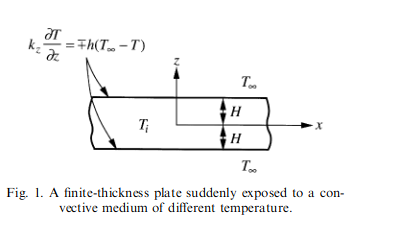
\includegraphics[]{fig1.png}
\begin{equation} \label{T_FS}
\frac{T(z,t) - T_i}{T_i - T_{\infty}} = -1 + 2 \sum ^{\infty} _{n=1} \exp(-\beta_n^2 \frac{k_z t}{H^2}) \times \frac{sin \beta_n cos(\beta_nz/H)}{\beta_n + sin \beta_n cos \beta_n} 
\end{equation}
Dimensionless stress distribution:
\[\sigma = 2 \sum ^{\infty} _{n=1} exp ( -\frac{(2n+1)^2\pi^2}{4} \frac{k_z t}{H^2} \times \left(\frac{(-1)^n}{2n+1} cos [\frac{(2n+1)\pi}{2} \frac{z}{H}] - \frac{2}{(2n+1)^2 \pi}\right) \]
where $k_z$ is the thermal diffusivity, $\beta_n$ are the roots of \[\beta_n tan \beta_n = Bi\]
and Biot number $Bi = hH/k$.  
%For UO2 pellets with radius of 0.0042 m, $h = 4.187 \times 10^3 W/m^2K$ \cite{UO2_thermal_shock}, $k = 5 W/mK$,  $Bi = \frac{rh}{k} = 3.5$.
H = 1m, h = $10000 W/m^2C$, k = 5 W/mC, thus, Bi = 2000.


\begin{center}
\begin{tabular}{ |c|c||c|c||c|c|| } 
 \hline
 $\beta_1$ & 1.57001 & $\beta_4$ & 10.9901 & $\beta_7$ & 20.4101 \\ 
 $\beta_2$ & 4.71003 & $\beta_5$ & 14.1301 & $\beta_8$ &  23.5502 \\ 
 $\beta_3$ & 7.85006 & $\beta_6$ & 17.2701 & $\beta_9$ & 26.6902 \\ 
 \hline
\end{tabular}
\end{center}

\section*{Results}
Fig. \ref{time_history} shows the temperature distribution from MOOSE at different periods of time after quenching in water bath.  
\begin{figure}[h]
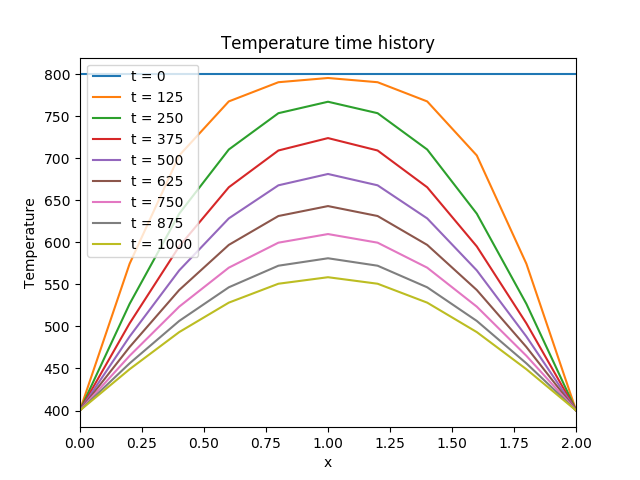
\includegraphics[]{T_time_history.png}
\caption{}
\label{time_history}
\end{figure}

Fig. \ref{fig:T}(a) - (d) show the Temperature profiles calculated from MOOSE have been compared to Fourier series approximation (Eq. \ref{T_FS}) 
\begin{figure}[h]
    \centering
    \begin{subfigure}[b]{0.4\textwidth}
        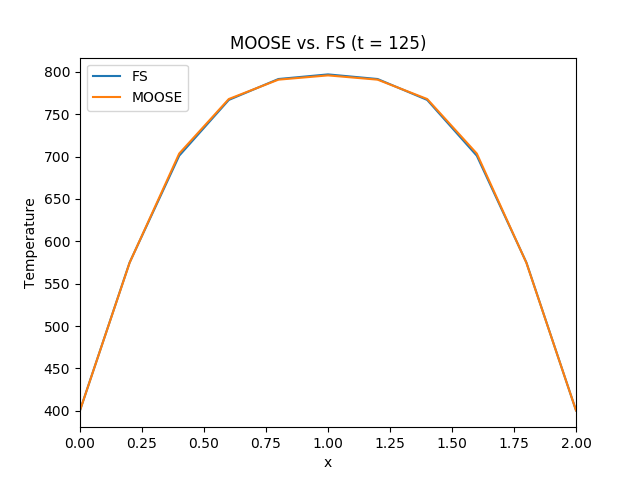
\includegraphics[width=\textwidth]{t125.png}
        \caption{t = 125 s}
        \label{fig:t125}
    \end{subfigure}
    ~ %add desired spacing between images, e. g. ~, \quad, \qquad, \hfill etc. 
      %(or a blank line to force the subfigure onto a new line)
    \begin{subfigure}[b]{0.4\textwidth}
        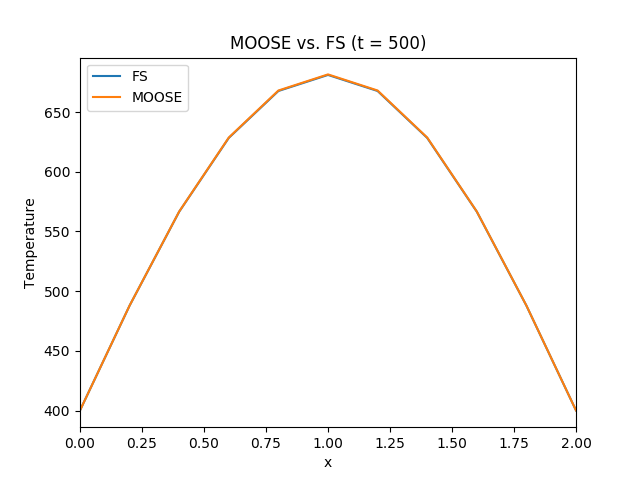
\includegraphics[width=\textwidth]{t500.png}
        \caption{t = 500 s}
        \label{fig:tiger}
    \end{subfigure}
    
    ~ %add desired spacing between images, e. g. ~, \quad, \qquad, \hfill etc. 
    %(or a blank line to force the subfigure onto a new line)
    \begin{subfigure}[b]{0.4\textwidth}
        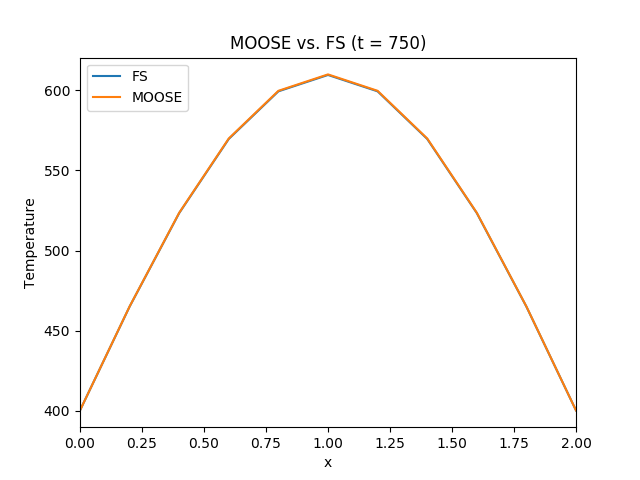
\includegraphics[width=\textwidth]{t750.png}
        \caption{t = 750 s}
        \label{fig:t750}
    \end{subfigure}
        \begin{subfigure}[b]{0.4\textwidth}
        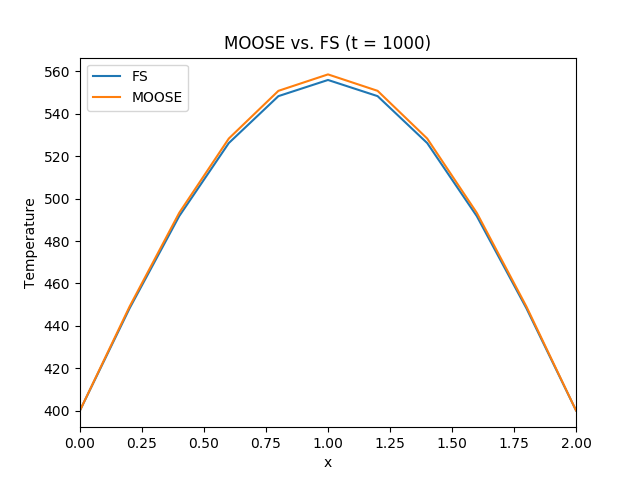
\includegraphics[width=\textwidth]{t1000.png}
        \caption{t = 1000}
        \label{fig:t1000}
    \end{subfigure}
    \caption{Pictures of animals}\label{fig:T}
\end{figure}


\begin{thebibliography}{9}
\bibitem{thermalShock_solid} 
T. J. Lu and N. A. Fleck, The thermal shock resistance of solid, Acta Mater., Vol. 46, No. 13, p. 4755 - 4768, 1998.
 
\bibitem{fracture_thermal_shock} 
H. A. Bahr, H. Balke, M. Kuna and H. Liesk
\textit{Fracture analysis of a single edge cracked strip under thermal shock}
Theoretical and Applied Fracture Mechanics, 8(1987) 33-39.
 
\bibitem{UO2_thermal_shock} 
Masaomi Oguma
\textit{Integrity degradation of UO2 pellets subjected to thermal shock}
Jounal of Nuclear Materials 127 (1985) 67-76.
\end{thebibliography}


\end{document}
